\documentclass[12pt,letterpaper,twoside]{article}
\usepackage[left=2cm,right=2cm,top=2cm,bottom=2cm]{geometry}
\usepackage[spanish]{babel}
%\usepackage[fixlanguage]{babelbib}
\usepackage{amsmath,amsfonts,amssymb,float}
\usepackage{kpfonts}
\usepackage{multicol}
\usepackage{enumitem}
\usepackage{authblk}
\usepackage{indentfirst}

%\usepackage[numbers]{natbib}

\usepackage[utf8]{inputenc}
\usepackage{mathrsfs}
\usepackage{fancyhdr,helvet}
\usepackage{units}
\usepackage{physics}
\usepackage{tikz}
\usepackage{caption}
\parindent=12.5pt
\decimalpoint

\newcommand{\helv}{\fontfamily{phv}\fontsize{9}{11}\selectfont}

\pagestyle{fancy}
\renewcommand{\sectionmark}[1]{\markright{\thesection\ #1}}
\fancyhf{}
\fancyfoot[LE,RO]{\helv\thepage}
\fancyhead[LO]{\helv\rightmark} 
\fancyhead[RE]{\helv J. Arias; A. Pineda; R. Gallardo.}

\usepackage{graphicx}
\usepackage{xcolor}

%\AtBeginDocument{\renewcommand\contentsname{Contenidos}}
\AtBeginDocument{\renewcommand\refname{Bibliografía}}  
\AtBeginDocument{\renewcommand\figurename{Figura}}  
\AtBeginDocument{\renewcommand\tablename{Cuadro}}  

\providecommand{\keywords}[1]{\textbf{\textit{Palabras clave:}} #1}

\title{Simulación numérica de la serie del actínido en GNU Octave con ecuaciones diferenciales estocásticas y Monte Carlo}

\author[$\dagger$]{J. Arias}
\author[$\dagger$]{A. Pineda}
\author[$\dagger$]{R. Gallardo}
\author[$*$]{F. Serrano}

\affil[$\dagger$]{\small Escuela de Física, Facultad de Ciencias, Universidad Nacional Autónoma de Honduras.\newline \textcolor{blue}{\{jmarias, apinedag, roberto.gallardo\}@unah.hn}}
\affil[$*$]{\small Instituto de Investigación en Energía, Universidad Nacional Autónoma de Honduras.}
%\affil[2]{\small Escuela de Física, Facultad de Ciencias, Universidad Nacional Autónoma de Honduras.\newline \textcolor{blue}{apinedag@unah.hn}}
%\affil[3]{\small Escuela de Física, Facultad de Ciencias, Universidad Nacional Autónoma de Honduras.\newline \textcolor{blue}{roberto.gallardo@unah.hn}}
\date{}

\begin{document}
\maketitle

        \begin{abstract}

\noindent Los elementos conocidos en la naturaleza muestran variaciones en su estructura nuclear. De especial interés son los radioisótopos; estos son átomos de un elemento que difieren del resto de su especie por el número de neutrones en su núcleo o por el nivel energético del mismo y que se desintegran hasta obtener una estructura estable. El uranio-235 es un radioisótopo natural. Su desintegración se suscita mediante una reacción en cadena en la que cada producto de fisión es inestable y se descompone en otro elemento en su debido turno. El modelo matemático que describe la reacción en cadena del U-235, también llamada serie del actínido, es las ecuaciones de Bateman. Para que la reacción en cadena tome lugar se requiere una masa mínima de material fisionable conocida como masa crítica. En cada proceso de desintegración se libera una cantidad de energía que puede transformarse en electricidad. Utilizamos GNU Octave para simular la serie del actínido mediante los métodos de Euler-Maruyama, Runge-Kutta y Monte Carlo. 
  
    \end{abstract}
    \keywords{Desintegración en cadena, serie del actínido, ecuaciones de Bateman, simulación numérica}

    \begin{center}
    \textbf{Objetivos}
\end{center}\vspace{-0.5cm}

\textbf{Objetivo general:}
\begin{itemize}
    \item Simular numéricamente en GNU Octave la desintegración en cadena
 del uranio-235.
\end{itemize}

\textbf{Objetivos particulares:}
\begin{itemize}
    \item Resolver completamente las ecuaciones de Bateman para la serie
 del actínido mediante los métodos de Euler-Maruyama, Runge-Kutta y Monte Carlo.
    \item Obtener una comparación de la eficiencia computacional de los métodos elegidos.
\end{itemize}
    
    \begin{center}
        \section*{Introducción} 
        \addcontentsline{toc}{section}{Introducción}
        \input{introduction}
    \end{center}

\begin{multicols}{2}
    
    \section{Energía nuclear y centrales nucleares}
        \subsection{Fisión y fusión nuclear}
    
Las reacciones nucleares —aquellas en las que participan los núcleos atómicos— pueden tener lugar espontáneamente, como en la radiactividad, o pueden ser inducidas por el bombardeo con una partícula o un haz. Las reacciones nucleares son mucho más
energéticas que las reacciones químicas, pero obedecen a las mismas leyes físicas: conservación de la cantidad de movimiento,
energía, número de partículas y carga. En la actualidad la cantidad de posibles reacciones nucleares es enorme, ya que existen aproximadamente 2000 isótopos conocidos y una gran cantidad de partículas que pueden ser utilizadas como proyectiles.  \cite{Murray.2020}\\
En una reacción nuclear, dos núcleos, o un nucleón, y un núcleo, se aproximan tanto que interactúan mediante la interacción fuerte. \cite{Cottingham.2001}\\ 
Una reacción nuclear se puede definir como una colisión entre dos núcleos que produce un
cambio en la composición nuclear y/o en el estado de energía de la interacción
núcleo. En circunstancias normales, las reacciones nucleares ocurren cuando un objetivo es bombardeado por partículas/núcleos provenientes de un acelerador o de una sustancia radiactiva.\\
Cuando dos núcleos o un núcleo y una partícula colisionan, Pueden ocurrir los siguientes escenarios: 
\begin{enumerate}
    \item \textbf{Dispersión} se da cuando el proyectil incidente se encuentra entre los resultados de la reacción. La dispersión puede ser:
    \begin{itemize}
        \item \textit{Elástica}: Se da cuando los núcleos que interactúan permanecen sin cambio y no se crean nuevas partículas. Solo existe una redistribución de las energías cinéticas de las partículas. Ejemplo:
        \begin{equation*}
            p+^{16}O \longrightarrow p+^{16}O
        \end{equation*}
        En este caso tanto el núcleo como el proyectil permanecen sin cambio, únicamente pueden cambiar la velocidad o la dirección de los elementos interactuantes. 
    \item \textit{Inelástica}: Se da cuando el núcleo o el proyectil se excitan después de la colisión, se fracturan formando nuevas partículas. En este tipo de reacciones parte de la energía cinética del sistema se convierte en energía interna. Ejemplo:
    \begin{equation*}
         n+^{16}O \longrightarrow n+^{16}O^*
    \end{equation*}
    El oxígeno termina en un estado excitado. 
    \end{itemize}
 \item \textbf{Transmutación} ocurre cuando se da un reordenamiento de los constituyentes nucleares dentro de los núcleos interactuantes. Ejemplo:
 \begin{equation*}
         d+^{14}N \longrightarrow ^{3}He+^{13}C
    \end{equation*}
\end{enumerate}
En esta reacción podemos observar como el núcleo de nitrógeno pierde un protón, convirtiéndose así en un núcleo de carbón. Mientras el núcleo de deuterio (d) adquiere este protón y se convierte en un núcleo de helio. 
Estas reacciones también pueden resultar en más de dos núcleos finales. Por ejemplo:
 \begin{equation*}
         \gamma+^{233}U \longrightarrow ^{90}Rb+^{141}Cs+2n
    \end{equation*}
Podemos observar en esta reacción que el núcleo de uranio se dividió en 2 núcleos más, más dos neutrones. \cite{Sanctis.2016}\\

Clasificaremos las reacciones nucleares existentes en dos grupos principales: reacciones de fisión y reacciones de fusión.



\subsubsection{Reacciones de Fisión}
La fisión es la ruptura espontánea o inducida de un núcleo. Si bien es “simplemente otra reacción” desde el punto de vista de la física, tiene un papel especial en asuntos públicos debido a sus enormes aplicaciones en la producción de energía y armamentos. \cite{Basdevant.2005}\\

En la fisión nuclear, el núcleo de un elemento pesado se divide en unos pocos
fragmentos más ligeros (generalmente dos, la llamada fisión binaria), liberando una gran cantidad de energía y un cierto número de neutrones libres (típicamente dos o tres). \cite{Murray.2020}
\begin{figure}[H]
    \centering
    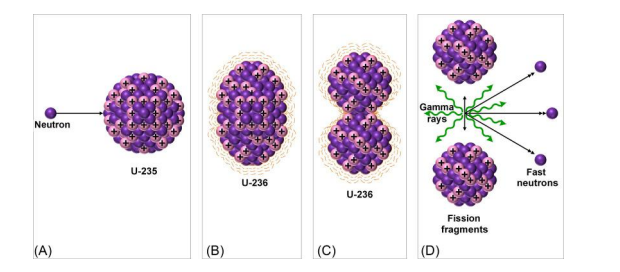
\includegraphics[scale=.55]{imagenes/fision nuclear.png}
    \caption{Proceso de fisión inducido, un neutrón interactúa con un núcleo de U-235, formando U-236, que luego se fisiona en dos partes, liberando energía y neutrones.\cite{Murray.2020}}
    \label{fig:fision}
\end{figure}
En comparación con reacciones químicas como la combustión de combustibles fósiles, la fisión requiere un volumen mucho menor de material combustible para producir una equivalente cantidad de energía. Para hacer la comparación más cuantitativa, la energía liberada por fisión de 1 gramo de U-235 es de unos 82 mil millones julios, equivalente a la liberada al quemar alrededor de tres millones gramos de carbón. \cite{Sanctis.2016}

\subsubsection{Reacciones de Fusión}
La fusión nuclear es la combinación de dos o más núcleos en un núcleo más pesado. Durante este proceso la suma de las masas de los constituyentes individuales es mayor que la masa del nuevo núcleo formado. Supongamos que se pueden combinar dos núcleos de hidrógeno y dos neutrones para
formar el núcleo de helio. En la reacción:
\begin{equation*}
    2^1_1H+2^1_0n \longrightarrow^4_2 He
\end{equation*}
El defecto de masa energía está dado por:
\begin{align}
    \nonumber \Delta m&=\Sigma M_{react}- M_{prod}\\
    \nonumber &=2M_{H-1}+2m_n-M_{He-4}\\
    \nonumber 0.030377&=2(1.007825)+2(1.008665)\\
    \nonumber &-4.002603\left[amu\right]
\end{align}
Lo que corresponde a 28.3 MeV de energía. \cite{Murray.2020}

Las reacciones de fusión, que tienen lugar en el Sol, siempre han sido la fuente principal de energía en la Tierra. En la Tierra, la vez que el humano manipuló esta energía fue en 1952, durante las pruebas de la bomba de hidrógeno. Desde entonces la humanidad ha tenido la ambición de domar esta forma de energía. Es más limpia que la fisión, creando muchos menos desechos radiactivos de vida larga. Sus recursos son ilimitados. En 300 litros de agua de mar hay 1 gramo de deuterio. El agua en los océanos podría proporcionar suficiente energía para las necesidades humanas durante varios cientos de millones de años. Es particularmente frustrante ver que, a diferencia de la fisión que se utilizó industrialmente unos años después de su descubrimiento, la fusión aún se encuentra en una etapa prospectiva más de 50 años después de su primer uso terrestre. \cite{Basdevant.2005}

Hasta ahora, un dispositivo práctico de energía de fusión no ha sido demostrado, y considerable investigación y desarrollo será necesario para alcanzar ese objetivo. \cite{Murray.2020}

\begin{figure}[H]
    \centering
    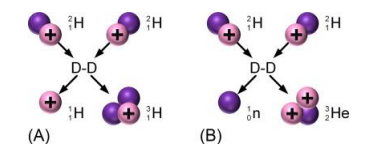
\includegraphics[scale=.65]{imagenes/fusion nuclear.png}
    \caption{Ejemplos de reacciones de fusión deuterio-deuterio (A) deuterio-deuterio (p) (B) deuterio-deuterio (n).\cite{Murray.2020}}
    \label{fig:fision}
\end{figure}
\subsection{Energía de desintegración}
Una reacción nuclear típica la podemos escribir como:
\begin{equation*}
  a + X \longrightarrow Y + b  
\end{equation*}
Aplicando conservación de la energía relativista podemos escribir la reacción como:
\begin{equation}
    m_Xc^2+T_x+m_ac^2+T_a\ \longrightarrow m_Yc^2+T_Y+m_bc^2+T_b
\end{equation}

Donde T representa la energía cinética de las partículas, en el ámbito no relativista podemos utilizar ($T=\frac{1}{2}mv^2$). Las m´s representan las masas en reposo de las partículas. Definiremos el valor Q (energía de la reacción o energía de desintegración) como:
\begin{equation}
    Q=(m_{inicial}-m_{final})c^2   
\end{equation}
También se puede expresar como el exceso de la energía final de los productos.
\begin{equation}
   Q=T_{final}-T_{inicial}
\end{equation} 
\begin{equation}
   Q=T_Y+T_b-T_X-T_a
\end{equation}
El valor de Q puede ser positivo o negativo. Si Q es negativo o cero, entonces se dice que la reacción es exotérmica. En este caso la masa nuclear o la energía de enlace se libera como energía cinética de los productos finales. Si el valor de Q es positivo, entonces la se dice que la reacción es endotérmica. En este caso la energía cinética inicial es convertida en masa nuclear o en energía de enlace. \cite{Krane.1987}
\subsection{Materiales fisionables}
La fisión de un núcleo en particular puede producir una gran cantidad de diferentes fragmentos. Por ejemplo para la captura neutrónica de un átomo de $^{235}U_{92}$ para formar $^{236}U_{92}$  podemos tener: \cite{Sanctis.2016}
\begin{figure}[H]
    \centering
    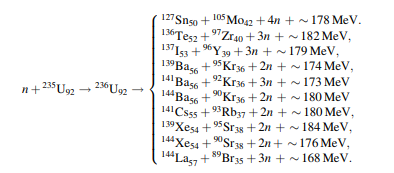
\includegraphics[scale=.925]{imagenes/posibilidades.png}
    \caption{Posibles resultados que se pueden obtener de la captura neutronica de $^{235}U_{92}$ para formar $^{236}U_{92}$.\cite{Sanctis.2016}}
    \label{fig:posibilidades}
\end{figure}        
Los núcleos pesados los cuales son estables o casi estables tienen una relación alta entre protones y neutrones a diferencia de los núcleos ligeros que tienden a tener aproximadamente la misma cantidad de neutrones y protones. Esta diferencia implica que al fisionarse los productos también serán ricos en neutrones. Por lo general lo productos de la fisión son inestables, poseyendo demasiados neutrones para un núcleo de su  numero másico, eventualmente decaerán mediante $\beta^-$ hasta formar un núcleo mas estable. 
\subsection{Tipos de centrales nucleares}
    
    \section{Desintegración nuclear}
        \subsection{Canales de decaimiento y tasas de ramificación}

\noindent Los canales de desintegración (\textit{decaimiento}) son los posibles cambios que puede tener una partícula a medida que se desintegra, estos se muestran en la figura \ref{channels}.

\begin{figure*}%[H]
    \begin{center}
        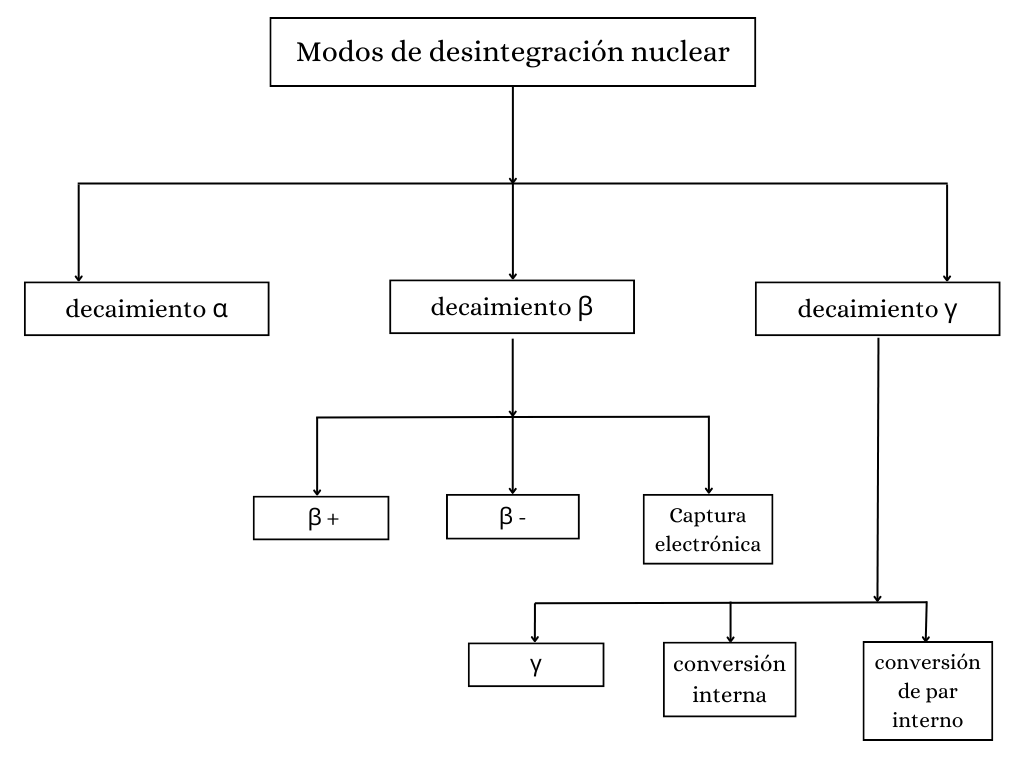
\includegraphics[scale=0.5]{imagenes/decay.png}
        \caption{Canales de desintegración para un radionúclido.}\label{channels}
    \end{center}
\end{figure*}

\noindent Según el tipo de átomo en cuestión, la desintegración radiactiva se produce a través de la emisión de diferentes tipos de radiaciones. Los principales son: 

\begin{itemize}
	\item Radiación alfa ($\alpha $):  la partícula emitida corresponde a un núcleo del elemento químico de helio. La masa del nuevo núcleo disminuye en cuatro unidades, con relación al núcleo inicial. Así, por ejemplo, cuando el átomo de uranio-238 emite una partícula alfa, se transforma en torio-234. La radiación alfa puede recorrer una distancia de apenas unos cuantos centímetros en el aire y puede ser detenida por una simple hoja de papel \cite{Krane.1987}.
	
	\item Radiación beta ($\beta $): la partícula emitida es un electrón. La masa del núcleo atómico formado no cambia con la transformación de un neutrón en un protón. Un neutrino (partícula elemental de carga cero y de masa extremadamente pequeña) se lleva la energía complementaría liberada en la transformación. La radiación beta puede recorrer una distancia de unos cuantos metros en el aire, y puede ser detenida con una placa de vidrio o de madera \cite{Krane.1987}. 
	
	\item Radiación gamma ($\gamma $): es un tipo de radiación electromagnética que transporta el exceso de energía de un núcleo inestable. La radiación gamma acompaña a las transformaciones radiactivas alfa y beta, y tiene un fuerte poder penetrante. Puede recorrer cientos de metros en el aire y se requiere de espesores importantes de plomo o cemento para detenerla \cite{Krane.1987}.
\end{itemize}

Los diversos modos de desintegración de un núcleo radiactivo son:

\begin{itemize}
	\item Decaimiento Alfa:
	
	En este proceso, el núcleo padre se desintegra para dar un núcleo hijo y una partícula $\alpha$ ($^{4} He$). El número de masa del núcleo hijo disminuye en cuatro unidades y el número atómico disminuye en dos unidades. Un ejemplo típico de este modo de caída es: 
	\begin{equation}
		^{238} _{92} U \longrightarrow \ ^{238} _{92} Th + ^{4} _{2} He
	\end{equation}
	
	\item Decaimiento Beta:
	
	En este proceso, el núcleo padre se desintegra para dar un núcleo hijo y una partícula $\beta $. Como se muestra en la figura 2, la desintegración $\beta $ se clasifica en tres categorías: 
	
    %	\begin{itemize}
    		\paragraph{Emisión de electrones o desintegración $\beta ^{-}$}: aquí, el núcleo padre se desintegra para dar un núcleo hijo, una partícula a $\beta ^{-}$ (o un electrón) y una nueva partícula llamada antineutrino. El número de masa del núcleo hijo permanece igual y el número atómico aumenta por una unidad. Un ejemplo es:
    	\begin{equation}
    		^{14} _{6} C \longrightarrow \ ^{14} _{7} N + \beta ^{-} + \bar{\nu }
    	\end{equation}
    	
    	\paragraph{Emisión de positrones o decaimiento $\beta ^{+}$}: en este proceso, el núcleo padre se desintegra para dar un núcleo hijo, una partícula $\beta ^{+}$ (o un positrón) y una nueva partícula llamada neutrino. El número de masa del núcleo hijo permanece igual y el número atómico disminuye en una unidad. Un ejemplo es:
    
    	\begin{equation}
    		^{22} _{11} Na \longrightarrow \ ^{22} _{10} Ne + \beta ^{+} + \nu 
    	\end{equation}
    	
    	\paragraph{Captura de electrones}: aquí el núcleo padre captura uno de los electrones orbitales con la emisión de un neutrino (n). El número de masa del núcleo hijo permanece igual y el número atómico disminuye en una unidad. Por ejemplo: 
    	
    	\begin{equation}
    		^{54} _{25} Mn + \beta ^{-}  \longrightarrow \  ^{54} _{24} Cr + \nu 
    	\end{equation}
    	
 %   	\end{itemize}
 
	\item Decaimiento Gamma:
	
	\noindent Si la energía de excitación disponible con un núcleo no es suficiente para la emisión de partículas, pierde su energía siguiendo tres procesos, como se muestra en la figura [\ref{channels}]. 
	
        \paragraph{Desintegración gamma}: las desintegraciones alfa y beta de un núcleo radiactivo suelen dejar al núcleo hijo en un estado excitado. Si la energía de excitación disponible con el núcleo hijo no es suficiente para una mayor emisión de partículas, pierde su energía al emitir radiaciones electromagnéticas, también conocidas como rayos g. La masa y la carga del núcleo hijo siguen siendo las mismas que antes de la emisión de rayos g. Un ejemplo es: 
    		\begin{equation}
    		^{137} _{56} Ba^{*} \longrightarrow \ ^{137} _{56} Ba + \gamma  
    		\end{equation}
    		El asterisco (*) en Ba indica que está en estado excitado o metaestable.
    		
    		\paragraph{Conversión interna}: en el proceso de conversión interna, un núcleo excitado en lugar de emitir rayos g transfiere directamente su energía de excitación a uno de los electrones orbitales y el electrón orbital es expulsado como electrón de conversión. La masa y la carga del núcleo hijo siguen siendo las mismas que antes de la emisión del electrón orbital. Esto es así porque se expulsa un electrón de las órbitas electrónicas.
    		\paragraph{Conversión de par interno}: si la energía de excitación del núcleo $>$ 1.022 MeV, el núcleo puede des-excitarse emitiendo directamente un par de electrones y positrones en su propio campo de Coulomb. Este proceso se conoce como conversión de pares internos \cite{Podgorsak.2016}.
\end{itemize}


\subsection{Probabilidades de decaimiento}

\noindent Las leyes de la desintegración radiactiva son: 
\begin{enumerate}
    \item Existe la misma probabilidad de que todos los núcleos de un elemento radiactivo se desintegran. 
 	
    \item La tasa de desintegración espontánea de un elemento radiactivo es proporcional al número de núcleos presentes en ese momento \cite{Krane.1987}.
 	
\end{enumerate}

\noindent Matemáticamente, se puede escribir como: 

\begin{equation}
    \frac{dN}{dt} \propto N
\end{equation}

\noindent donde N es el número de átomos presentes en el tiempo t. Eliminando el signo de proporcionalidad, obtenemos: 

\begin{equation}
\frac{dN}{dt} = -\lambda N\label{ecuaciondiferencialN}
\end{equation} 

\noindent Donde $\lambda $ es una constante de proporcionalidad y se conoce como constante de decaimiento del elemento. El signo negativo indica que a medida que t aumenta, N disminuye. Reescribiendo la ecuación \ref{ecuaciondiferencialN} como: 

\begin{equation}
\frac{dN}{N} = -\lambda dt
\end{equation} 

\noindent Integrando ambos lados tenemos: 

\begin{equation}
ln( \lambda ) = -\lambda t + C\label{ecuacionlambda}
\end{equation}

\noindent donde C es una constante de integración y se evalúa por el hecho de que en t = 0, el número de átomos del elemento radiactivo es $N_0$. Usando esta condición, obtenemos: 

\begin{equation}
    C = ln (N_0)
\end{equation}

\noindent Sustituyendo este valor de C en la ecuación \ref{ecuacionlambda}: 

\begin{equation}
    ln\left( \frac{N}{N_0} \right) = - \lambda t 
\end{equation}

\noindent Con esto tenemos que: 

\begin{equation}
    N = N_{0} e^{ - \lambda t }
\end{equation}

\noindent La naturaleza exponencial de esta ecuación muestra que se necesita un tiempo infinito para que todo el material radiactivo se desintegre. N versus t se ha representado gráficamente para $ ^{24} Na$ ($t_{1/2} = 15h$) en la figura \ref{decaimientodelsodio24}. Una gráfica de $log(N)$ frente a $t$ sería una línea recta.

\begin{figure*}
    \begin{center}
        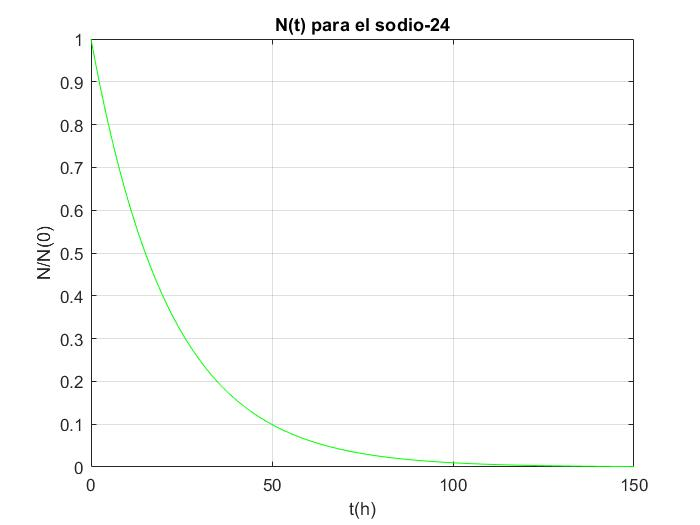
\includegraphics[scale=0.5]{imagenes/decaimiento_sodio_24.jpg}
        \caption{Gráfica del decaimiento exponencial del sodio-24 en en un intervalo de 150 horas.}
        \label{decaimientodelsodio24}
    \end{center}
\end{figure*}

\subsection{Desintegración en cadena}


\subsection{Ecuaciones de Bateman}

\noindent Las ecuaciones de Bateman son un sistema de ecuaciones diferenciales ordinarias propuestas por el matemático británico Harry Bateman en 1910 para generalizar las cadenas de desintegración del tipo $Padre\rightarrow Hijo \rightarrow Nieto$ \cite{Podgorsak.2016}.

\noindent Debido a que la cantidad de núcleos que participan en el proceso de desintegración es tan grande, podemos suponer que la función $N=N(t)$ que da el número de núcleos en un tiempo $t$ es una función continua, no discreta. De esta manera, es posible aplicar sobre ella las reglas de cálculo como ya las conocemos \cite{Podgorsak.2016}. 

\noindent Siguiendo a \textit{Podgorsak} en \cite{Podgorsak.2016}, tenemos que la cadena de desintegración descrita en el modelo de Bateman comprende las siguientes condiciones iniciales:

\begin{equation}
    \eval{N_1(t)}_{t=0}=N_1(0)\neq 0,\label{condicioninicialpadre}
\end{equation}
\begin{equation}
    N_2(0)=N_3(0)=...=N_i(0)=0, \label{condicioninicialproductos}
\end{equation}

\noindent como conveniencia para futuras referencias llamaremos a la ecuación \ref{condicioninicialpadre} \textit{condición inicial del núcleo padre} y a \ref{condicioninicialproductos}, \textit{condición inicial de los productos}. 

\noindent El significado o la implicación de las ecuaciones \ref{condicioninicialpadre} y \ref{condicioninicialproductos} es que, en un tiempo inicial, $t=0$, únicamente disponemos de los núcleos de la muestra padre para desintegración nuclear, mientras que los productos de su fisión permanecen inexistentes. Es solo hasta que el padre ha decaído que comenzamos a ver valores de $N$ distintos de cero para los elementos resultantes de la fisión. 

\noindent El número de núcleos disponibles en un tiempo $t$ para el k-ésimo producto de fisión viene dado por:

\begin{equation}
        N_k(t)=N_1(0) e^{-\lambda_1 t}+C_2 e^{-\lambda_2 t}+...+C_k e^{-\lambda_k t} \label{iesimonucleo}
\end{equation}

\noindent Donde $N_1^{(0)}$ es el número inicial de núcleos de la muestra radiactiva. Para los valores numéricos de los coeficientes $C_k$ de Bateman, \textit{Flanagan y Senftle} en \cite{Flanagan1954} ofrecen tablas completas de los términos que involucran.

En general, \cite{Loch.2013} ofrece una generalización más compacta válida para cualquier núcleo en la secuencia:

\begin{equation}
        N_m(t)=N_1^{(0)} \prod_{k=1}^{m-1}\lambda_k\sum_{j=1}^{m}\left(\frac{e^{\lambda_j t}}{\prod\limits_{p=1, p\neq j}^{m}\left(\lambda_p-\lambda_j\right)}\right) \label{batemangeneral}
\end{equation}

\noindent De acuerdo con \textit{Pratiwi et al} en \cite{Pratiwi.2021}, Bateman habría resuelto sus ecuaciones con transformadas de Laplace, y este método sería efectivo para sistemas lineales \textit{bien portados}, pero en el caso de reacciones en cadena con bifurcaciones en los productos de desintegración sumado a constantes de desintegración diferentes para cada producto, el sistema requiere de un tratamiento matricial numérico. 

En la sección \ref{actinidoserie} se desarrolla el esquema matricial en el caso particular para la cadena del uranio-235. 
       
    \section{Serie del actínido}\label{actinidoserie}
        La desintegración en cadena  del $^{235} U$ se conoce como la serie del actínido \cite{Podgorsak.2016}. Como parte del proceso de desintegración radiactiva, los productos de fisión del uranio emiten neutrones y rayos gamma al atravesar una serie de decaimientos beta \cite{Guo.2016}. La causa de esta serie de desintegraciones nucleares se debe a la razón de neutrones sobre protones, es mediante el canal beta que estos núcleos logran la estabilidad \cite{Guo.2016}. 

De acuerdo con \textit{Guo et al} en \cite{Guo.2016}, al momento de analizar una cadena de desintegración compleja se simplifica el problema al resolver la reacción a través de reacciones lineales en las que cada núcleo está relacionado solo a un núcleo madre; el núcleo madre puede estar en su estado base o en un estado excitado, partiendo de esto llamamos a cada cadena lineal \textit{la del estado base} y \textit{la del estado excitado}, respectivamente.

El proceso de desintegración del uranio-235 contempla bifurcaciones en varios puntos, esto es: hay productos de desintegración que pueden a su vez producir uno de dos posibles núcleos más estables \cite{HUBENER2003211, International_Atomic_Energy_Agency2013-bq}. La literatura observa más o menos bifurcaciones para el proceso, como podemos apreciar en \cite{HUBENER2003211,International_Atomic_Energy_Agency2013-bq,Pratiwi.2021,Loch.2013}, por mencionar tres ejemplos. Para mantener la simulación lo más fiel posible al proceso real, tomamos como referencia la cadena presentada por \textit{Hübener} en \cite{HUBENER2003211}, la cual está ilustrada en la imagen \ref{cadenadelu235}.

\begin{figure}[H]
    \centering
    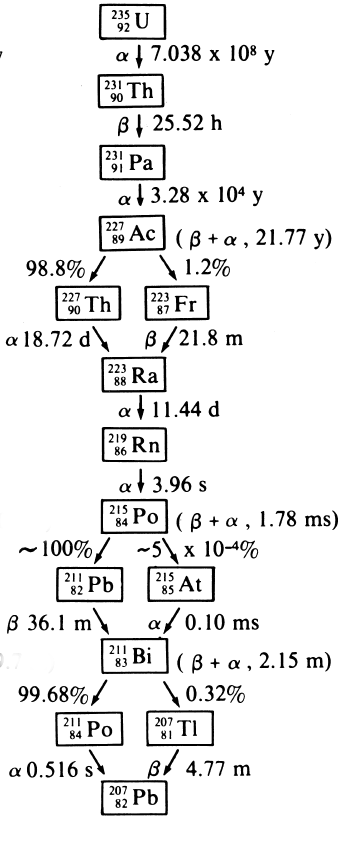
\includegraphics[scale=0.425]{imagenes/cadenaluz.png}
    \caption{Cadena de desintegración del U235 hasta Pb207. Tomada de \cite{HUBENER2003211}}.
    \label{cadenadelu235}
\end{figure}

Contemplar el proceso de enriquecimiento del material fisionable complica en gran manera la resolución del problema, es por esto que ignoraremos esta etapa del proceso.  

\subsection{Ecuaciones de Bateman para la serie del actínido}

Es posible modelar las ecuaciones de Bateman en una notación matricial contemplando un sistema de ecuaciones para cada posible bifurcación \cite{Pratiwi.2021}. Nuestra intención en este estudio es más bien contemplar las bifurcaciones mediante un modelo diferencial estocástico.

Tomando en cuenta las condiciones iniciales \ref{condicioninicialpadre} y \ref{condicioninicialproductos} y la forma de $N_i(t)$ en \ref{iesimonucleo}, podemos plantear las ecuaciones de Bateman de la siguiente forma:
\begin{align}
    N_1'(t)&=-\lambda_1 N_1(t)\\ \label{ecubateman1}
    N_2'(t)&=\lambda_1 N_1(t) -\lambda_2 N_2(t)\\
    N_3'(t)&=\lambda_2 N_2(t) -\lambda_3 N_3(t)\\
    N_4'(t)&=\lambda_3 N_3(t) -\lambda_4 N_4(t)\\
    N_5'(t)&=(1-f_4)\lambda_4 N_4(t) -\lambda_5 N_5(t)\\
    N_6'(t)&=f_4 \lambda_4 N_4(t) -\lambda_6 N_6(t)\\
    N_7'(t)&=\lambda_6 N_6(t) + \lambda_5 N_5(t) -\lambda_7 N_7(t)\\
    N_8'(t)&=\lambda_7 N_7(t) -\lambda_8 N_8(t)\\
    N_9'(t)&=\lambda_8 N_8(t) -\lambda_9 N_9(t)\\
    N_{10}'(t)&=\lambda_9 N_9(t) -\lambda_{10} N_{10}(t)\\
%\end{align}
%
%\begin{align}
    N_{11}'(t)&=\lambda_{10} N_{10}(t) -\lambda_{11} N_{11}(t)\\
    N_{12}'(t)&=(1-f_{11})\lambda_{11} N_{11}(t) -\lambda_{12} N_{12}(t)\\
    N_{13}'(t)&=f_{11}\lambda_{11}N_{11}(t) -\lambda_{13} N_{13}(t)\\
    N_{14}'(t)&=\lambda_{12} N_{12}(t) + \lambda_{13} N_{13}(t)
    \label{ecubateman14}
\end{align}

\noindent donde $f_k$ son tasas de ramificación. Las $N_i(t)$ se definen de la siguiente manera:
\begin{itemize}
    \item $N_1(t)\equiv$ \textit{Núcleos de} $^{235}U$.
    \item $N_2(t)\equiv$ \textit{Núcleos de} $^{231}Th$.
    \item $N_3(t)\equiv$ \textit{Núcleos de} $^{231}Pa$.
    \item $N_4(t)\equiv$ \textit{Núcleos de} $^{227}Ac$.
    \item $N_5(t)\equiv$ \textit{Núcleos de} $^{227}Th$
    \item $N_6(t)\equiv$ \textit{Núcleos de} $^{223}Fr$
    \item $N_7(t)\equiv$ \textit{Núcleos de} $^{223}Ra$.
    \item $N_8(t)\equiv$ \textit{Núcleos de} $^{219}Rn$.
    \item $N_9(t)\equiv$ \textit{Núcleos de} $^{215}Po$.
    \item $N_{10}(t)\equiv$ \textit{Núcleos de} $^{211}Pb$
    \item $N_{11}(t)\equiv$ \textit{Núcleos de} $^{211}Bi$.
    \item $N_{12}(t)\equiv$ \textit{Núcleos de} $^{211}Po$
    \item $N_{13}(t)\equiv$ \textit{Núcleos de} $^{207}Tl$.
    \item $N_{14}(t)\equiv$ \textit{Núcleos de} $^{207}Pb$
\end{itemize}

\noindent para los factores de ramificación tenemos:
\begin{itemize}
    \item $f_4=\frac{\lambda_{4,\alpha}}{\lambda_{4,\alpha}+\lambda_{4,\beta}}$, donde $\lambda_{4,\alpha}$ es la tasa de desintegración del $^{227}Ac$ hacia $^{223}Fr$, mientras que $\lambda_{4,\beta}$ representa la tasa de desintegración de $^{227}Ac$ hacia $^{227}Th$. 
    \item $f_{11}=\frac{\lambda_{11,\alpha}}{\lambda_{11,\alpha}+\lambda_{11,\beta}}$, donde $\lambda_{11,\alpha}$ es la tasa de desintegración del $^{211} Bi$ hacia $^{207} Tl$, mientras que $\lambda_{11,\beta}$ representa la tasa de desintegración de $^{211} Bi$ hacia $^{211} Po$.
\end{itemize}

Para obtener las tasas de ramificación es preciso conocer los valores de las constantes de decaimiento en cada canal del radionúclido. Si conocemos la probabilidad de desintegración mediante un canal dado y la vida media del radionúclido, es posible calcular $\lambda_{i,\alpha}$ y $\lambda_{i,\beta}$ para el iésimo núcleo con:

$$\lambda_{i,canal}=\frac{\textrm{Probablidad del canal}}{\tau_i}$$

De acuerdo con los archivos de \textit{National Nuclear Data Center}, las probabilidades para el canal alfa y el beta en el Ac-227 son, respectivamente, 0.0138 y 0.9862. Las probabilidades para el canal alfa y el beta en el Bi-211 son, respectivamente, 0.99724 y 0.00276. De manera que $f_4=0.01380$ y $f_{11}=0.99724$.

La constante de decaimiento $\lambda_i$ para el i-ésimo núcleo es una función del período de semidesintegración $T_{1/2}^{(i)}$, estos valores son conocidos y están documentados en la literatura, tal es el caso de \cite{Flanagan1954}. La tabla \ref{tabladeconstantesdedesintegracion} muestra las constantes de decaimiento de cada núcleo en las ecuaciones \ref{ecubateman1} hasta \ref{ecubateman14} junto con el período de semidesintegración que le concierne según estos registros. 

%\begin{minipage}{\textwidth}
%\begin{table}[h]
%    \centering
\begin{center}
\noindent\begin{tabular}{|c|l|l|}
\hline
Radionúclido & \multicolumn{1}{c|}{$T_{1/2}$} & \multicolumn{1}{c|}{$\lambda\ (a^{-1})$} \\\hline\hline 
$^{235}U$ & $7.13\times10^8$ a & $9.7216\times 10^{-10}$ \\
$^{231}Th$ & 26.64 h & $2.2793\times 10^{2}$ \\
$^{231}Pa$ & 34 300 a & $2.0208\times 10^{-5}$ \\
$^{227}Ac$ & 22.0 a & $3.1507\times 10^{-2}$ \\
$^{227}Th$ & 18.6 d & $1.3602\times 10^{1}$ \\
$^{223}Fr$ & 21 min & $1.7348\times 10^{4}$ \\
$^{223}Ra$ & 11.2 d & $2.2589\times 10^{1}$ \\
$^{219}Rn$ & 3.92 s & $5.5763\times 10^{6}$ \\
$^{215}Po$ & $1.83\times10^{-3}$ s & $1.1945\times 10^{10}$ \\
$^{211}Pb$ & 36.1 min & $1.0092\times 10^{4}$ \\
$^{211}Bi$ & 2.16 min & $1.6867\times 10^{5}$ \\
$^{211}Po$ & 0.52 s & $4.2037\times 10^{7}$ \\
$^{207}Tl$ & 4.79 min & $7.6058\times 10^{4}$ \\
$^{207}Pb$ & Estable & \\\hline
\end{tabular}
\captionof{table}{Períodos de semidesintegración y constantes de decaimiento para cada radionúclido en la cadena del uranio-235. Datos según \cite{Flanagan1954}.}
\label{tabladeconstantesdedesintegracion}
%\end{table}
%\end{minipage}
\end{center}

Hay que señalar que en este modelo, las ecuaciones de Bateman tienen una forma determinista. Bajo la perspectiva de un modelo estocástico diferencial, vemos que la solución del sistema sería la solución esperada para el caso determinista más un término perturbativo que es en sí una variable aleatoria dependiente del tiempo. 

En la literatura se reportan métodos analíticos para resolver sistemas de ecuaciones como el planteado aquí empleando transformadas de Laplace o exponenciales de matrices. En el presente, utilizamos el método de eigenvectores para establecer la solución general del sistema. Al notar que el sistema de ecuaciones puede representarse con una ecuación matricial de la forma

$$\mathbf{N'}(t)=\Lambda \mathbf{N}(t)$$

Donde $\mathbf{N}(t)$ es un vector cuyas componentes son las funciones $N_i(t)$ y $\mathbf{N'}(t)$ es el vector que contiene sus derivadas. La matriz $\Lambda$ es triangular inferior de dimensión $14\times14$, dada como \ref{matriz_determinista} en los anexos.

%\begin{minipage}{\textwidth}
%\begin{equation}
%\begin{smallmatrix}
%        -\lambda_1 &  &  &  &  &  &  &  &  &  &  &  &  \\
%        \lambda_1 & -\lambda_2 &  &  &  &  &  &  &  &  &  &  &  \\
%         & \lambda_2 & -\lambda_3 &  &  &  &  &  &  &  &  &  &  \\
%         &  & \lambda_3 & -\lambda_4 &  &  &  &  &  &  &  &  &  \\
%         &  &  & (1-f_4)\lambda_4 & -\lambda_5 &  &  &  &  &  &  &  &  \\
%         &  &  & f_4\lambda_4 &  & -\lambda_6 &  &  &  &  &  &  &  \\
%         &  &  &  & \lambda_5 & \lambda_6 & -\lambda_7 &  &  &  &  &  &  \\
%         &  &  &  &  &  & \lambda_7 & -\lambda_8 &  &  &  &  &  \\
%         &  &  &  &  &  &  & \lambda_8 & -\lambda_9 &  &  &  &  \\
%         &  &  &  &  &  &  &  & \lambda_9 & -\lambda_{10} &  &  &  \\
%         &  &  &  &  &  &  &  &  & \lambda_{10} & -\lambda_{11} &  &  \\
%         &  &  &  &  &  &  &  &  &  & (1-f_{11})\lambda_{11} & -\lambda_{12} &  \\
%         &  &  &  &  &  &  &  &  &  & f_{11}\lambda{11} &  & -\lambda_{13} \\
%         &  &  &  &  &  &  &  &  &  &  & \lambda_{12} & f_{13}\lambda{13} 
%    \end{smallmatrix}
%\end{equation}    
%\end{minipage}

De tal forma que las soluciones del sistema vienen dados como combinación lineal de los eigenvectores de $\Lambda$:

$$\mathbf{N}(t)=\kappa_1 e^{-\lambda_1 t} \mathbf{V}_{\lambda_1}+\kappa_2 e^{-\lambda_2 t} \mathbf{V}_{\lambda_2}+...+\kappa_{14} e^{-\lambda_{14} t} \mathbf{V}_{\lambda_{14}}$$

\noindent Las constantes de integración $K_i$ son determinadas por las condiciones iniciales $\mathbf{N}(0)=\left[N_1^{(0)}\ 0\ 0\ ...\ 0\right]^T$.

\subsubsection{Cálculo de los coeficientes de Bateman}

De acuerdo con la ecuación \ref{batemangeneral}, podemos emplear las constantes de decaimiento en el cuadro \ref{tabladeconstantesdedesintegracion} para determinar los coeficientes de Bateman de la serie del actínido. Resumimos los resultados en el cuadro \ref{tabla_coeficientes_bateman1} y \ref{tabla_coeficientes_bateman2}. 

Donde $C_k^*=C_k/N_1^{(0)}$. Estos resultados han de reemplazarse en las soluciones deterministas para trazar las gráficas del decaimiento de cada una de las muestras resultantes en la cadena, así como del núcleo padre. Al encontrar las soluciones deterministas tenemos un acercamiento al perfil que tendrán las soluciones estocásticas. 

Por otro lado, los coeficientes obtenidos en el método de eigenvectores están resumidos en el cuadro \ref{tabladecoeficientes2}. 

\begin{center}
\begin{tabular}{|c|r|}
    \hline
    k-ésimo coeficiente & \multicolumn{1}{c|}{valor aproximado}\\\hline\hline
    $\kappa_1^*$ & 1.4142  \\
    $\kappa_2^*$ & $-6.0319\times 10^{-12}$ \\
    $\kappa_3^*$ & $-6.8060\times 10^{-5}$ \\
    $\kappa_4^*$ & $2.8055\times 10^{-11}$ \\
    $\kappa_5^*$ & $-2.5284\times 10^{-16}$ \\
    $\kappa_6^*$ & $2.0738\times 10^{-6}$ \\
    $\kappa_7^*$ & $-3.9435\times 10^{-16}$ \\
    $\kappa_8^*$ & $-6.1232\times 10^{-19}$ \\
    $\kappa_9^*$ &  $-1.0091\times 10^{-19}$ \\
    $\kappa_{10}^*$ & $5.7702\times 10^{-19}$ \\
    $\kappa_{11}^*$ & $7.2150\times 10^{-20}$ \\
    $\kappa_{12}^*$ & $-5.9116\times 10^{-19}$ \\
    $\kappa_{13}^*$ & $0.0000$ \\
    $\kappa_{14}^*$ & $1.0000$ \\
    \hline
\end{tabular}
\captionof{table}{Coeficientes de Bateman mediante método de eigenvectores.}\label{tabladecoeficientes2}
\end{center}

\subsection{Modelo estocástico matricial}


    \section{Implementación en GNU Octave}
        \subsection{Método de Runge-Kutta Estocástico}

\subsection{Método de Euler-Maruyama}

\subsection{Monte Carlo}
        
    \section{Análisis y discusión de los resultados}
        \input{section5_analisis_discusion}

    \section{Conclusiones}
        \input{conclusion}

\end{multicols}
    \section{Anexos}
        \subsection{Matrices del sistema}
La matriz $\Lambda$ de coeficientes de desintegración del sistema es un arreglo disperso. A continuación se muestra dejando en blanco aquellos elementos valuados en 0:

\begin{equation}
	\Lambda=\left(\begin{smallmatrix}
		-\lambda_1& & & & & & & & & & & & & & \\
		 \lambda_1&-\lambda_2& & & & & & & & & & & & & \\
		 & \lambda_2&-\lambda_3& & & & & & & & & & & & \\
		 & & \lambda_3&-\lambda_4& & & & & & & & & & & \\
		 & & &\lambda_{4,\beta}&-\lambda_5& & & & & & & & & & \\
		 & & &\lambda_{4, \alpha}& &-\lambda_6& & & & & & & & & \\
		 & & & & \lambda_5& \lambda_6&-\lambda_7& & & & & & & & \\
		 & & & & & & \lambda_7&-\lambda_8& & & & & & & \\
		 & & & & & & & \lambda_8&-\lambda_9& & & & & & \\
		 & & & & & & & &\lambda_{9,\alpha}&-\lambda_{10}& & & & & \\
		 & & & & & & & &\lambda_{9, \beta}& &-\lambda_{11}& & & & \\
		 & & & & & & & & & \lambda_{10}&\lambda_{11}&-\lambda_{12}& & & \\
		 & & & & & & & & & & &\lambda_{12, \beta}&-\lambda_{13}& & \\
		 & & & & & & & & & & &\lambda_{12, \alpha}& &-\lambda_{14}& \\ 
		 & & & & & & & & & & & &\lambda_{13}&\lambda_{14}& 0\\
	\end{smallmatrix}\right)
\end{equation}\label{matriz_determinista}

Para la versión estocástica del sistema, se toma como término determinista la matriz $\mathcal{L}$ y las matrices estocásticas $\mathcal{X}$, $\mathcal{Y}$ y $\mathcal{Z}$ dadas por los siguientes arreglos dispersos:

\begin{equation}
	\mathcal{L}=\left(\begin{smallmatrix}
		-\lambda_1& & & & & & & & & & & \\								%fila 1
		\lambda_1&-\lambda_2& & & & & & & & & & \\						%fila 2
		&\lambda_2&-\lambda_3& & & & & & & & & \\						%fila 3
		& & \lambda_3&-\lambda_4& & & & & & & & \\						%fila 4
		& & &\lambda_{4, \alpha}&-\lambda_6& & & & & & & \\				%fila 5
		& & & &\lambda_6 &-\lambda_7& & & & & & \\						%fila 6
		& & & & &\lambda_7&-\lambda_8& & & & & \\						%fila 7
		& & & & & &\lambda_8&-\lambda_9& & & & \\						%fila 8
		& & & & & & &\lambda_{9, \beta}&-\lambda_{11}& & & \\			%fila 9
		& & & & & & & &\lambda{11}&-\lambda_{12}& & \\					%fila 10
		& & & & & & & & &\lambda_{12, \beta}&-\lambda_{14}&\\			%fila 11 
		& & & & & & & & & &\lambda{14}& 0\\								%fila 12
	\end{smallmatrix}\right)
\end{equation}\label{matriz_determinista_alternativa}

\begin{equation}
	\mathcal{X}=\begin{cases}
		(\lambda_4-2\lambda_{4, \alpha}) & \textrm{En la fila 5, columna 4.}\\
		-\lambda_5+\lambda_6 & \textrm{En la fila 5, columna 5.}\\
		\lambda_5-\lambda_6 & \textrm{En la fila 6, columna 5.}
	\end{cases}
\end{equation}\label{matriz_estocastica_x}

\begin{equation}
	\mathcal{Y}=\begin{cases}
		-(\lambda_9-2\lambda_{9, \alpha}) & \textrm{En la fila 9, columna 8.}\\
		-\lambda_{10}+\lambda_{11} & \textrm{En la fila 9, columna 9.} \\
		\lambda_{10}-\lambda_{11} & \textrm{En la fila 10, columna 9.} \\
	\end{cases}
\end{equation}\label{matriz_estocastica_y}

\begin{equation}
	\mathcal{Z}=\begin{cases}
		(\lambda_{12}-2\lambda_{12, \alpha}) & \textrm{En la fila 11, columna 10.}\\
		-\lambda_{13}+\lambda_{14} & \textrm{En la fila 11, columna 11.}\\
		\lambda_{13}-\lambda_{14}  & \textrm{En la fila 12, columna 11.}\\
	\end{cases}
\end{equation}\label{matriz_estocastica_z}

\noindent donde se suponen 0 todos los elementos no especificados.

\subsection{Tablas de coeficientes}
A continuación se presentan los coeficientes obtenidos para la serie del actínido mediante la simulación por GNU Octave bajo el esquema de eigenvectores. 
\begin{center}
\begin{tabular}[h]{|c|r|r|r|r|}
    \hline
    $N_i$ & $C_1^*$ & $C_2^*$ & $C_3^*$ & $C_4^*$  \\\hline\hline
    $N_1$ & $1.00000000$ & $0$ & $0$ & $0$ \\
    $N_2$ & $5.51288098\times 10^{-7}$& $-5.51288098\times 10^{-7}$ & $0$ & $0$ \\
    $N_3$ & $4.65333818\times 10^{-5}$& $5.57897907\times 10^{-7}$ & $-4.70912797\times 10^{-5}$ & $0$ \\
    $N_4$ & $3.09248238\times 10^{-8}$& $3.92796956\times 10^{-10}$ & $-3.13163987\times 10^{-8}$ & $-1.22207337\times 10^{-12}$ \\
    $N_5$ & $1.00429565\times 10^{-12}$& $1.27579176\times 10^{-14}$ & $-1.01701378\times 10^{-12}$ & $-3.97809227\times 10^{-17}$ \\
    $N_6$ & $5.86387844\times 10^{-14}$& $7.44810663\times 10^{-16}$ & $-5.93812778\times 10^{-14}$ & $-2.31726572\times 10^{-18}$ \\
    $N_7$ & $4.44937366\times 10^{-11}$& $5.65191533\times 10^{-13}$ & $-4.50571672\times 10^{-11}$ & $-1.76087766\times 10^{-15}$ \\
    $N_8$ & $1.78377969\times 10^{-16}$& $2.26588562\times 10^{-18}$ & $-1.80636795\times 10^{-16}$ & $-7.05946067\times 10^{-21}$ \\
    $N_9$ & $8.02482795\times 10^{-20}$& $1.01937152\times 10^{-21}$ & $-8.12644752 \times 10^{-20}$ & $-3.17589429 \times 10^{-24}$ \\
    $N_{10}$ & $9.75861373\times 10^{-14}$& $1.23960972\times 10^{-15}$ & $-9.88218850\times 10^{-14}$ & $-3.86206702\times 10^{-18}$ \\
    $N_{11}$ & $1.03599574\times 10^{-26}$& $1.31599652\times 10^{-28}$ & $-1.04911471\times 10^{-26}$ & $-4.10004175\times 10^{-31}$ \\
    $N_{12}$ & $5.78523143\times 10^{-15}$& $7.34881961\times 10^{-17}$ & $-5.85849067\times 10^{-15}$ & $-2.28956247\times 10^{-19}$ \\
    $N_{13}$ & $2.31805658\times 10^{-17}$& $2.94456320\times 10^{-19}$ & $-2.34741047\times 10^{-17}$ & $-9.17393781\times 10^{-22}$ \\
    $N_{14}$ & $3.55803094\times 10^{-17}$& $4.51966849 \times 10^{-19}$ & $-3.60308682\times 10^{-17}$ & $-1.40812647\times 10^{-21}$ \\
    $N_{15}$ & $-1.00004712$& $-7.00318644\times 10^{-9}$ & $4.71226424\times 10^{-5}$ & $1.22388044\times 10^{-12}$ \\
    \hline
\end{tabular}
\captionof{table}{Coeficientes de Bateman obtenidos mediante eigenvectores. Parte 1}\label{tabla_coeficientes_bateman1}
\end{center}

\begin{center}
\begin{tabular}[h]{|c|r|r|r|r|}
    \hline
   $N_i$ & $C_5^*$ & $C_6^*$ & $C_7^*$ & $C_8^*$  \\\hline\hline
   $N_1$ & $0$& $0$ & $0$ & $0$ \\
   $N_2$ & $0$& $0$ & $0$ & $0$ \\
   $N_3$ & $0$& $0$ & $0$ & $0$ \\
   $N_4$ & $0$& $0$ & $0$ & $0$ \\
   $N_5$ & $0$& $4.88856388\times 10^{-25}$ & $0$ & $0$ \\
   $N_6$ & $9.50138278\times 10^{-30}$ & $0$ & $0$ & $0$ \\
   $N_7$ & $-9.51409697\times 10^{-30}$ & $7.69096154\times 10^{-25}$ & $4.78609631\times 10^{-24}$ & $0$ \\
   $N_8$ & $-3.82573383\times 10^{-35}$ & $3.08335862\times 10^{-30}$ & $1.91878144\times 10^{-29}$ & $1.90321436\times 10^{-32}$ \\
   $N_9$ & $-1.72111485\times 10^{-38}$ & $1.38713444\times 10^{-33}$ & $8.63217083\times 10^{-33}$ & $8.56599161\times 10^{-36}$ \\
   $N_{10}$ & $3.26399237\times 10^{-32}$ & $1.68909355\times 10^{-27}$ & $1.05202483\times 10^{-26}$ & $-1.90755340\times 10^{-32}$ \\
   $N_{11}$ & $-2.22193897\times 10^{-45}$ & $1.79077407\times 10^{-40}$ & $1.11440298\times 10^{-39}$ & $1.10588725\times 10^{-42}$ \\
   $N_{12}$ & $2.14355861\times 10^{-33}$ & $1.00143055\times 10^{-28}$ & $6.23756480\times 10^{-28}$ & $3.59322574\times 10^{-35}$ \\
   $N_{13}$ & $8.59228100\times 10^{-36}$ & $4.01258523\times 10^{-31}$ & $2.49930117\times 10^{-30}$ & $1.65548072\times 10^{-37}$ \\
   $N_{14}$ & $1.68328476\times 10^{-35}$ & $6.16008576\times 10^{-31}$ & $3.83733666\times 10^{-30}$ & $-3.10073991\times 10^{-39}$ \\
   $N_{15}$ & $-2.20564442\times 10^{-32}$& $-1.25974588\times 10^{-24}$ & $-4.79726585\times 10^{-24}$ & $-1.27035860\times 10^{-36}$ \\
        \hline
\end{tabular}
\captionof{table}{Coeficientes de Bateman obtenidos mediante mediante eigenvectores. Parte 2}\label{tabla_coeficientes_bateman2}
\end{center}

\begin{center}
	\begin{tabular}[h]{|c|r|r|r|r|}
		\hline
		$N_i$ & $C_9^*$ & $C_{10}^*$ & $C_{11}^*$ & $C_{12}^*$  \\\hline\hline
		$N_1$ & $0$& $0$ & $0$ & $0$ \\
		$N_2$ & $0$& $0$ & $0$ & $0$ \\
		$N_3$ & $0$& $0$ & $0$ & $0$ \\
		$N_4$ & $0$& $0$ & $0$ & $0$ \\
		$N_5$ & $0$& $0$ & $0$ & $0$ \\
		$N_6$ & $0$ & $0$ & $0$ & $0$ \\
		$N_7$ & $0$ & $0$ & $0$ & $0$ \\
		$N_8$ & $0$ & $0$ & $0$ & $0$ \\
		$N_9$ & $-2.88467470\times 10^{-35}$ & $0$ & $0$ & $0$ \\
		$N_{10}$ & $2.88467044\times 10^{-35}$ & $0$ & $-2.17703376\times 10^{-29}$ & $0$ \\
		$N_{11}$ & $-3.94554377\times 10^{-42}$ & $3.04250308\times 10^{-42}$ & $0$ & $0$ \\
		$N_{12}$ & $4.65721718\times 10^{-41}$ & $-3.04250545\times 10^{-42}$ & $-1.37194870\times 10^{-30}$ & $-1.08392039\times 10^{-30}$ \\
		$N_{13}$ & $-6.46462136\times 10^{-46}$ & $2.36278724\times 10^{-48}$ & $-5.49850503\times 10^{-33}$ & $-4.36062925\times 10^{-33}$ \\
		$N_{14}$ & $-1.78300791\times 10^{-48}$ & $6.53807648\times 10^{-51}$ & $-9.72206436\times 10^{-33}$ & $5.4271346\times 10^{-33}$ \\
		$N_{15}$ & $2.23180703\times 10^{-48}$ & $-4.57859868\times 10^{-52}$ & $2.31575069\times 10^{-29}$ & $1.08285388\times 10^{-30}$ \\
		\hline
	\end{tabular}
	\captionof{table}{Coeficientes de Bateman obtenidos mediante mediante eigenvectores. Parte 3}\label{tabla_coeficientes_bateman3}
\end{center}

\begin{center}
	\begin{tabular}[h]{|c|r|r|r|}
		\hline
		$N_i$ & $C_{13}^*$ & $C_{14}^*$ & $C_{15}^*$ \\\hline\hline
		$N_1$ & $0$& $0$ & $0$ \\
		$N_2$ & $0$& $0$ & $0$ \\
		$N_3$ & $0$& $0$ & $0$ \\
		$N_4$ & $0$& $0$ & $0$ \\
		$N_5$ & $0$& $0$ & $0$ \\
		$N_6$ & $0$ & $0$ & $0$ \\
		$N_7$ & $0$ & $0$ & $0$ \\
		$N_8$ & $0$ & $0$ & $0$ \\
		$N_9$ & $0$ & $0$ & $0$ \\
		$N_{10}$ & $0$ & $0$ & $0$ \\
		$N_{11}$ & $0$ & $0$ & $0$ \\
		$N_{12}$ & $0$ & $0$ & $0$ \\
		$N_{13}$ & $4.76594956\times 10^{-34}$ & $0$ & $0$ \\
		$N_{14}$ & $0$ & $-1.20997671\times 10^{-32}$ & $0$ \\
		$N_{15}$ & $-4.76594956\times 10^{-34}$& $1.20997671\times 10^{-32}$ & $1.00000000$ \\
		\hline
	\end{tabular}
	\captionof{table}{Coeficientes de Bateman obtenidos mediante mediante eigenvectores. Parte 4}\label{tabla_coeficientes_bateman4}
\end{center}

\subsection{Gráficas de las soluciones del sistema}
Se presentan las gráficas de las soluciones generadas por Octave en el marco de eigenvectores. 

\begin{figure}[H]
	\centering
	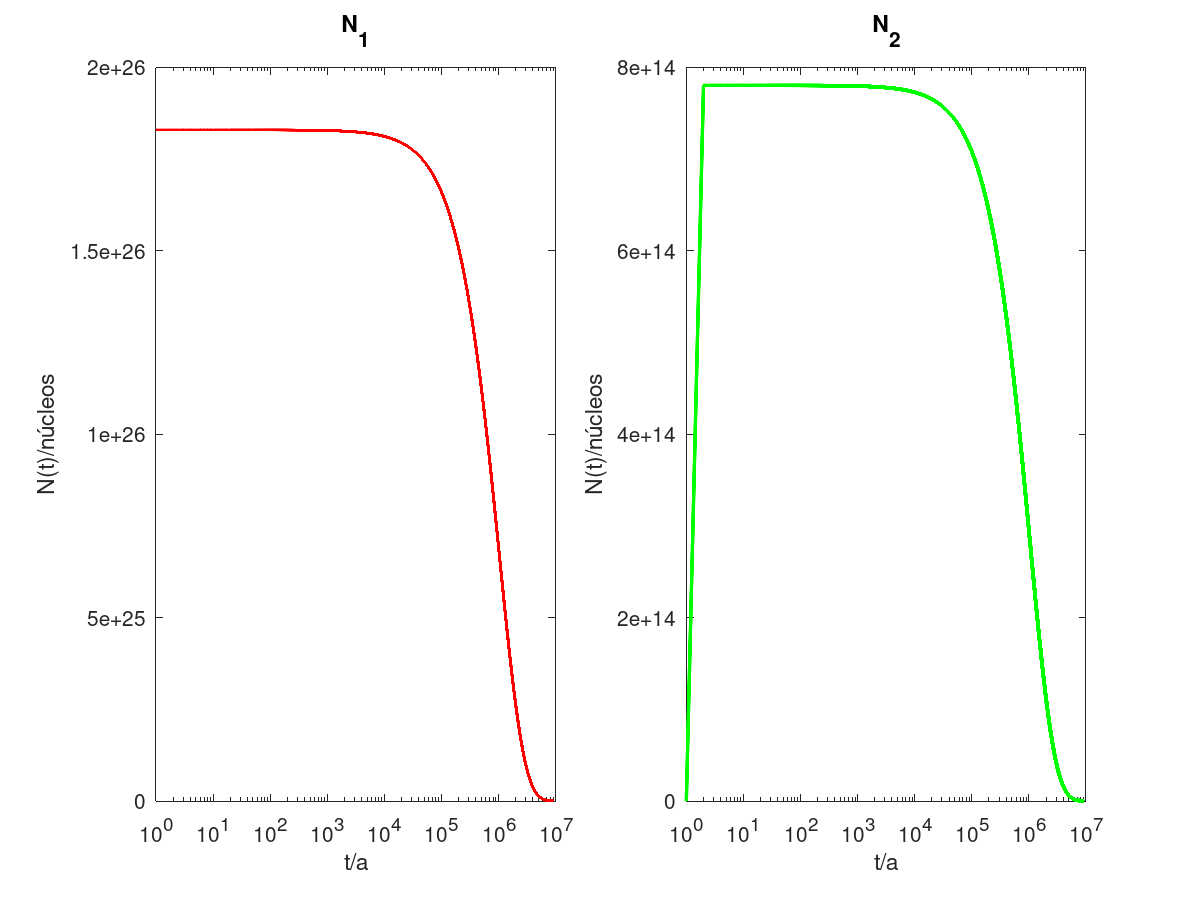
\includegraphics[scale=0.33]{/home/arias/Desktop/Research/u235_decay_chain_numsim/figuras/n1_n2.png}\label{n1n2}\caption{Curvas de desintegración de los núcleos $N_1$ y $N_2$ generadas por GNU Octave.}
\end{figure}

\begin{figure}[H]
	\centering
	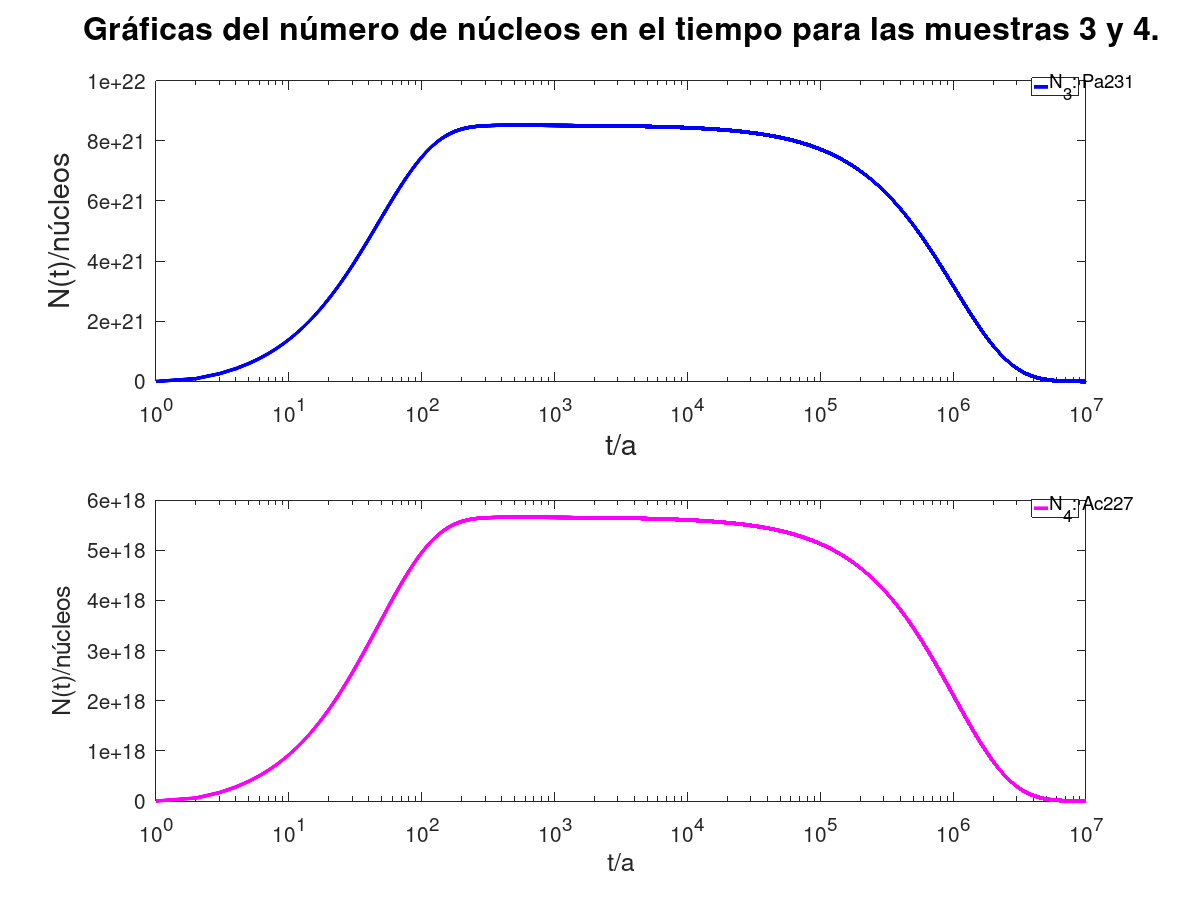
\includegraphics[scale=0.33]{/home/arias/Desktop/Research/u235_decay_chain_numsim/figuras/n3_n4.png}\label{n3n4}\caption{Curvas de desintegración de los núcleos $N_3$ y $N_4$ generadas por GNU Octave.}
\end{figure}

\begin{figure}[H]
	\centering
	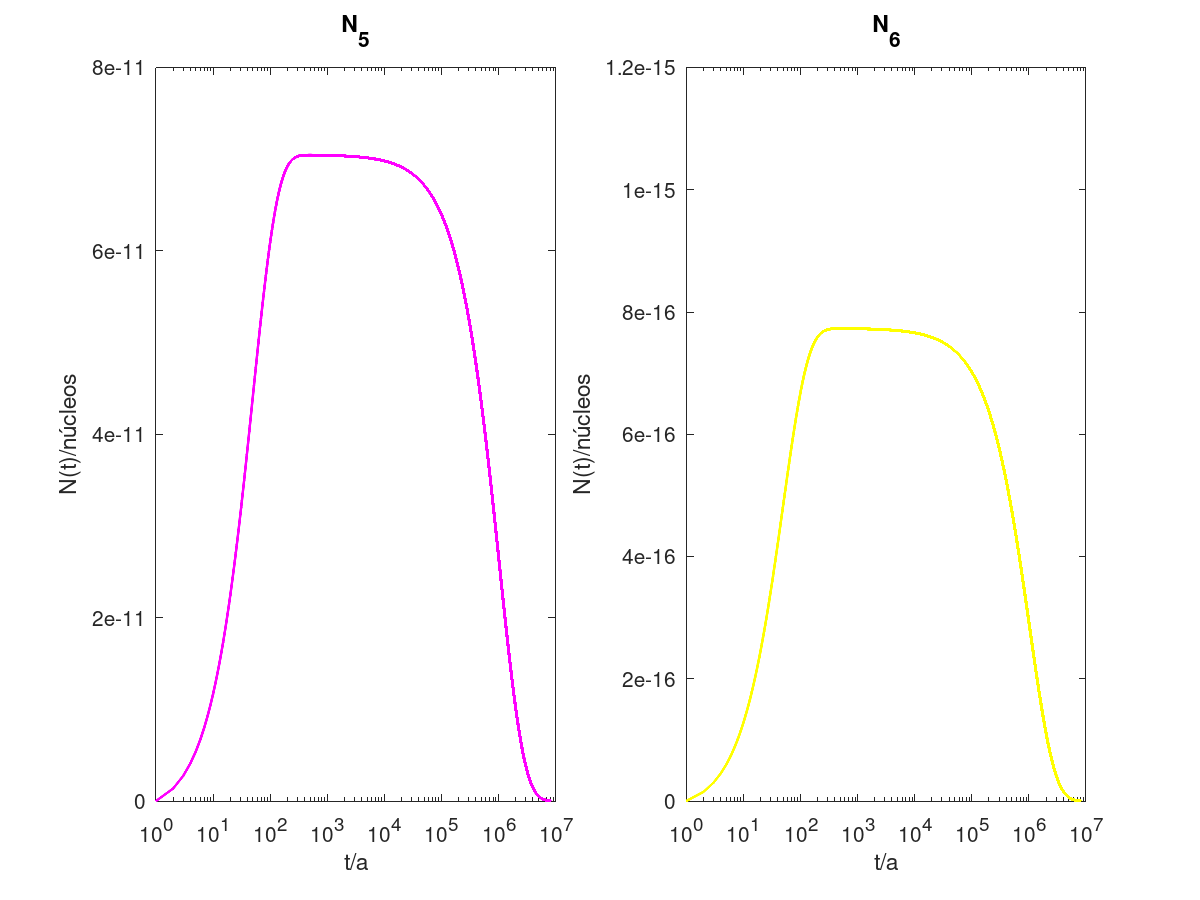
\includegraphics[scale=0.33]{/home/arias/Desktop/Research/u235_decay_chain_numsim/figuras/n5_n6.png}\label{n5n6}\caption{Curvas de desintegración de los núcleos $N_5$ y $N_6$ generadas por GNU Octave.}
\end{figure}

\begin{figure}[H]
	\centering
	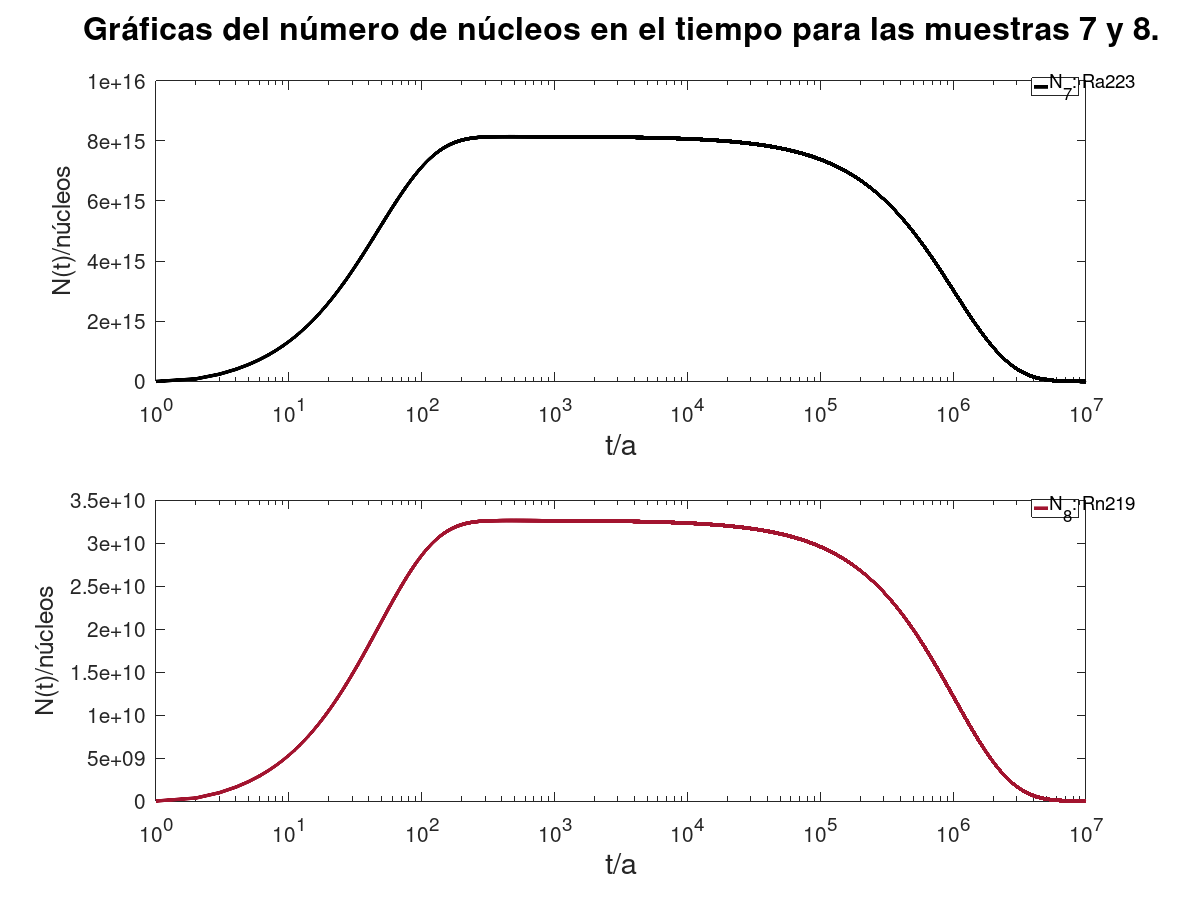
\includegraphics[scale=0.33]{/home/arias/Desktop/Research/u235_decay_chain_numsim/figuras/n7_n8.png}\label{n3n4}\caption{Curvas de desintegración de los núcleos $N_7$ y $N_8$ generadas por GNU Octave.}
\end{figure}

\begin{figure}[H]
	\centering
	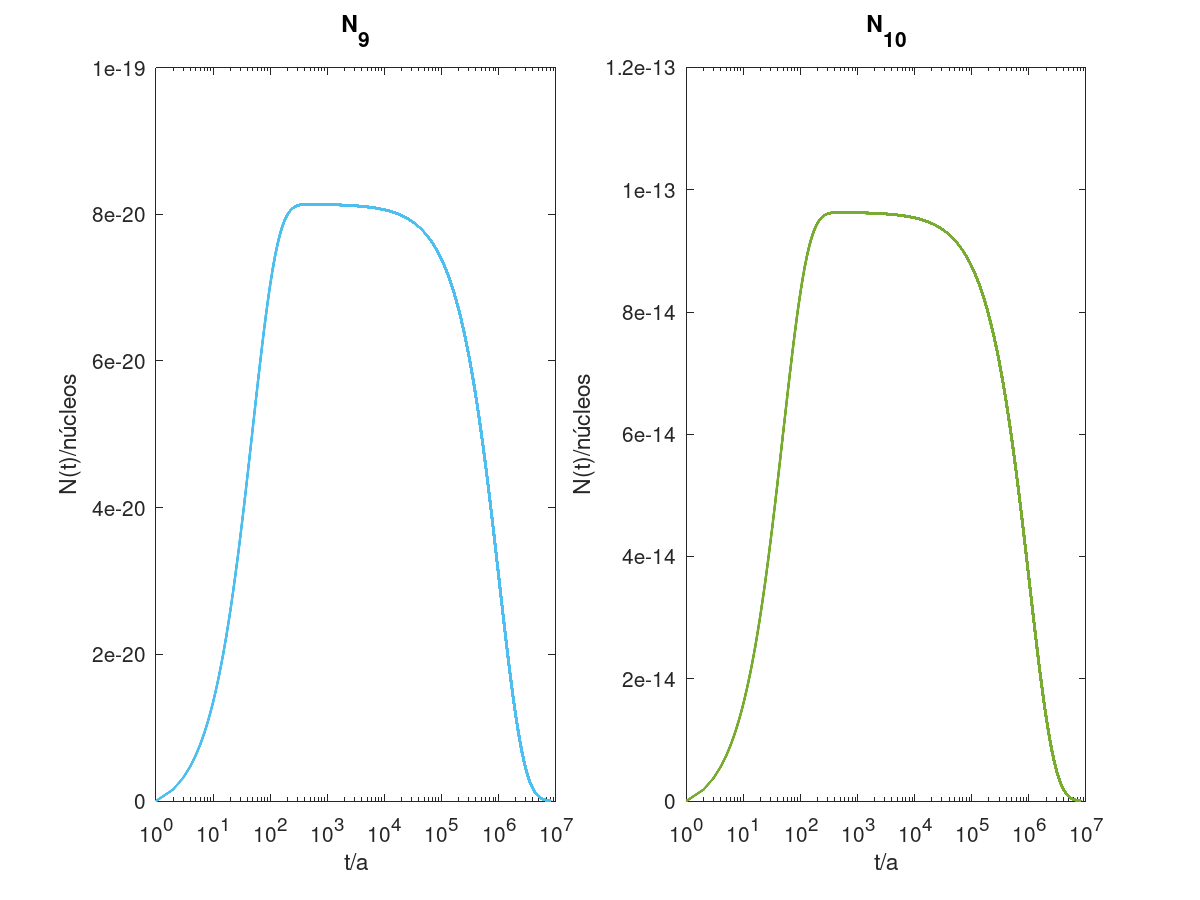
\includegraphics[scale=0.33]{/home/arias/Desktop/Research/u235_decay_chain_numsim/figuras/n9_n10.png}\label{n3n4}\caption{Curvas de desintegración de los núcleos $N_9$ y $N_{10}$ generadas por GNU Octave.}
\end{figure}

\begin{figure}[H]
	\centering
	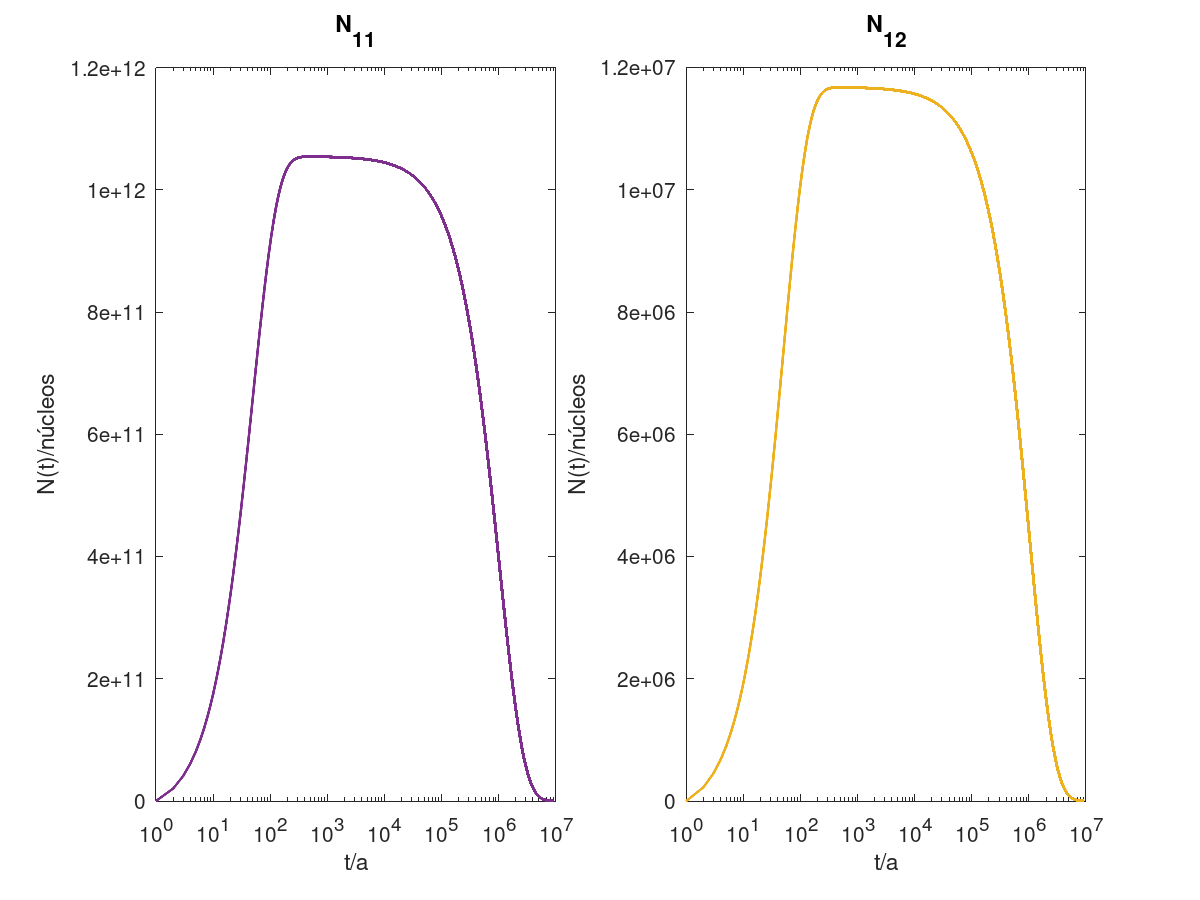
\includegraphics[scale=0.33]{/home/arias/Desktop/Research/u235_decay_chain_numsim/figuras/n11_n12.png}\label{n3n4}\caption{Curvas de desintegración de los núcleos $N_{11}$ y $N_{12}$ generadas por GNU Octave.}
\end{figure}

\begin{figure}[H]
	\centering
	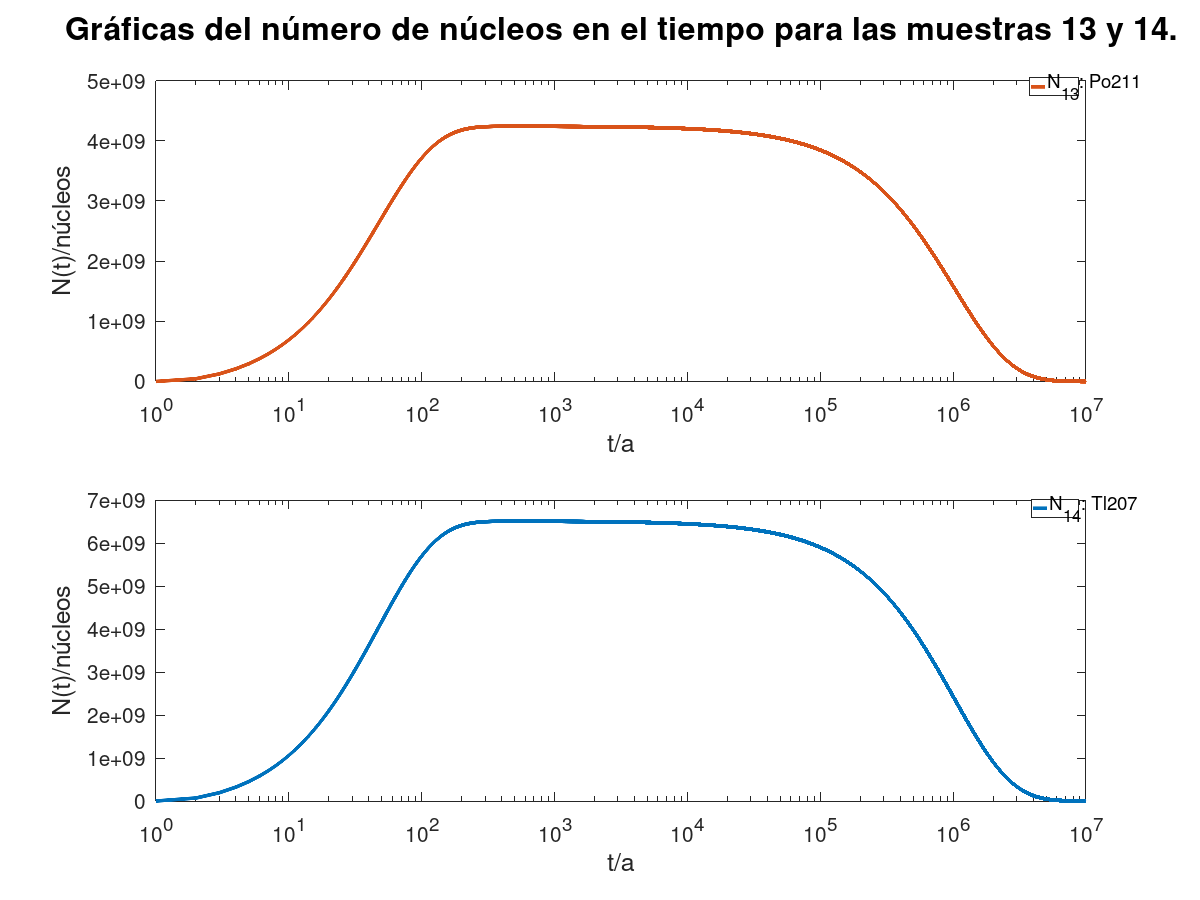
\includegraphics[scale=0.33]{/home/arias/Desktop/Research/u235_decay_chain_numsim/figuras/n13_n14.png}\label{n3n4}\caption{Curvas de desintegración de los núcleos $N_{13}$ y $N_{14}$ generadas por GNU Octave.}
\end{figure}

\begin{figure}[H]
	\centering
	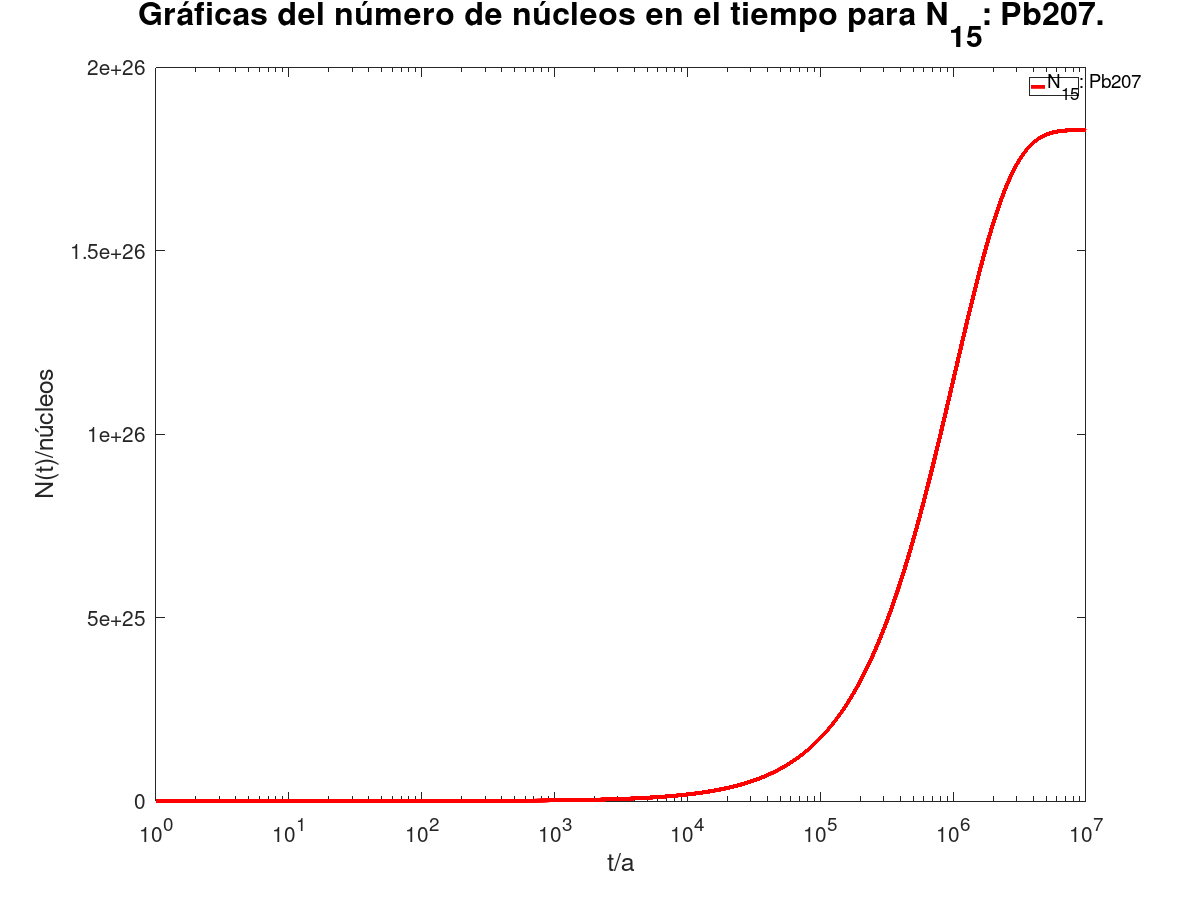
\includegraphics[scale=0.33]{/home/arias/Desktop/Research/u235_decay_chain_numsim/figuras/n15.png}\label{n15}\caption{Curva de desintegración del núcleo $N_{15}$ generada por GNU Octave.}
\end{figure}

\newpage

\nocite{Basdevant.2005} 
\nocite{Cottingham.2001} 
\nocite{Das.2009} 
\nocite{Eidemuller.2021} 
\nocite{Krane.1987} 
\nocite{Martin.2009} 
\nocite{Meyers.2018} 
\nocite{Murray.2020} 
\nocite{Sanctis.2016} 
\nocite{Serrano.2020} 
\nocite{Podgorsak.2016} 
\nocite{Eidemuller.2021} 
\nocite{Guo.2016} 
\nocite{Koizumi.2021} 
\nocite{Loch.2013} 
\nocite{Pratiwi.2021}
\nocite{MoralesBolio.1974}

\bibliographystyle{ieeetr}
\bibliography{proyecto_iie_energia_nuclear.bib}

\end{document}
